\chapter{Bearleaders}

Bearleaders is the name of a project I was assigned as soon as I arrived in the company. It was a project born thanks to a friendship between Wienke and a good friend of him, who basically became our client. This project was supposed to be my main mission within the Smiths, with a duration of at least two months, up to four.

\medskip

For several years, she (the client) had been running a small business: \textbf{a website gathering all the points of interest in the main cities of Europe}. The spots were sorted by categories (food, sleep, bars, ...). Anyone was able to sign up on this website and add spots, letting other users see them. Consequently, logged in users were able to browse across all the spots uploaded by users, get details, comment, etc. It was a kind of guide for Europe, on the Internet. Its main advantage was that it was free with a fairly important community.

\medskip

But some day, she came to Wienke with an idea in mind, knowing what \textsc{The Smiths} was. She wanted to "upgrade" her website and push her business to the next level. \textbf{Actually, she wanted a mobile app to replace her aging website, available on iOS and Android.}

\medskip

Both Wienke and her agreed on a time frame of two months, for a really fair price. The road map was pretty simple:

\begin{enumerate}
  \item Understanding the need
  \item Designing the mobile app while writing specifications
  \item Coding
  \item Tests, improvements and publishing
\end{enumerate}

This was an entire project from scratch. \textbf{We had to create the back-end\footnote{Everything related to the distant server, which generally stores data and provides services to clients (such as a mobile app or a website). It is usually made of a database and an API.}, take care of the old database and create a new one, develop the API and a back-office as well. In parallel, we were obviously also responsible for the development of the mobile app on Android and iOS.}

\section{Understanding the need}

When I arrived, in early September 2015, Wienke told me I would be in charge of the entire project, working jointly and closely with our designer, Wessel \textsc{Versluis}. However, after a couple of days, I had met the client only once, whereas Wienke and Wessel had many times. I found that quite weird as I was supposed to be responsible for the project. The only reason I had been given was that me attending the meetings was not necessary at that stage. Later, I understood that they were actually trying to figure out what the client really expected from us.

\medskip

Finally, after a few weeks, I had a better understanding of the project, the idea behind it, the final goal, and so forth. Thanks to the tight collaboration between Wessel and me, things were starting to move progressively. As I said above, the client wanted a fresh new version of her website made available as a mobile app.

\medskip

After being granted access to the old codebase of her website, it turned out to be rather obsolete and unmaintainable, regarding the frameworks used and the general quality. The database was a mess as well, really hard to maintain. I could foresee a huge amount of work coming ahead of me. In addition, she wanted most of the existing features to be somehow exported to the app, as well as adding brand new features.

\section{Designing the app}

In late September, meetings were still scheduled on a regular basis, but only involving Wessel and the client. These were mainly about design concerns. As for me, things were quite clear, from a technical point a view solely. However, after every meeting, I was getting news from Wessel about new features to add or remove. As far as I am concerned, I found it really inappropriate. In my opinion, the client was just overthinking and could not help herself from that. She was merely unable to agree on an ultimate product because of a poorly prepared plan.

\medskip

Wessel did a really good job figuring out which features were fundamental and which ones were not. He also proved a great ability to sketch mockups quickly, providing me with PNG exports as soon as the client would agree on them.

\medskip

On my side, I was designing the whole architecture of the project with everyone else's help, to finally start writing down the specifications.

\section{Specifications}

At some point, I had enough clues to start writing the specifications, although we still had not agreed on anything completely definitive. The contract was non-existent, which I though was not a good sign whatsoever.

\medskip

It had been decided to host the back-end source code on \href{https://www.parse.com}{parse.com}, and build the API on top of that. In addition, we would obviously use Titanium as a mobile app development platform for the mobile app, enabling us to use the same codebase for both Android and iOS.

\medskip

\href{https://www.parse.com}{Parse.com} offers, for free (with certain conditions, but it fitted our needs perfectly), a whole hosting solution and a set of tools to deploy server code flawlessly, thanks to a CLI. Moreover, they also provide their database made in-house, which in fact is a sort of more abstracted layer, on top of a regular database underneath (MongoDB\footnote{A database management system (DBMS) slightly different from conventional systems (relational systems)}). Parse is marketed as a BaaS\footnote{\textit{Back-end As A Service}} but it can be considered as a PaaS\footnote{\textit{Platform As A Service}} since the tech stack is very similar to other service providers like \href{https://www.heroku.com/}{Heroku}. Just like on any regular hosting provider, one can deploy source code simply by typing a command in a terminal. In the code, communication with Parse's database is established thanks to an API (a few JavaScript functions) provided by Parse, called "Cloud Code"\footnote{\href{https://parse.com/docs/cloudcode/guide}{https://parse.com/docs/cloudcode/guide}}.

\medskip

Regarding the API, as our whole stack relies on JavaScript, we naturally decided to go with \href{http://expressjs.com/}{Express.js} which is one of the greatest minimalist frameworks, used to build APIs insanely fast, in solely a couple of lines. Besides, it is even natively embedded in Parse, which means that Parse can run an Express.js server.

\begin{figure}[!h]
   \centering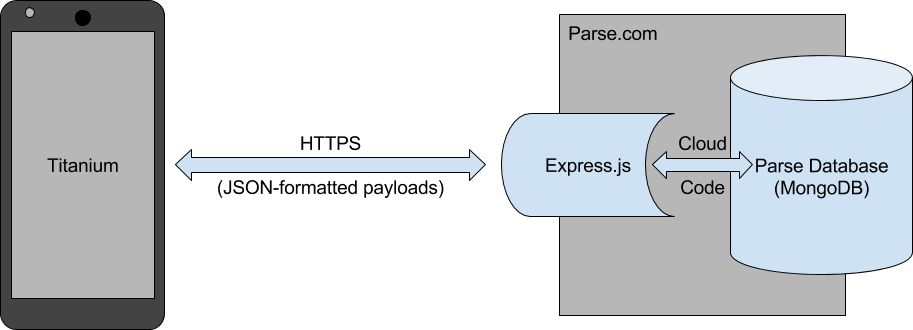
\includegraphics[width=1.00\textwidth]{images/bearleaders.png}
   \caption[Bearleaders' architecture]{Bearleaders' architecture}
\end{figure}

\section{API}

While writing specifications, I identified different type of entities (for example \textit{users}, \textit{spots}, \textit{categories}). As I wanted the API to be serviceable and convenient, I decided to reflect the entities through the API. That was the time I made loads of research about APIs and eventually ended up writing a blog post\footcite[See the reference][in the bibliography]{api_my_blog} about that topic, which has massively contributed to the writing of chapter \ref{chap:api}, in this report.

\medskip

I will not explain any further how I built the API as everything has already been told in the chapter \ref{chap:api}. As a matter of fact, the only purpose of that API was solely to reflect and expose the underlying database, allowing logged-in users and administrators to perform additions or edits, depending on their rights.

\section{Exporting the old database to the new back-end}

Upon completion of the specifications, I was focused on the development of the API. I was going back and forth as I would notice problems or potential issue in my design. Then came the tricky part.

\medskip

This part was not easy at all and yet, really interesting. From a MySQL\footnote{A popular database management system (DBMS)} dump sent to me by our client, I had to export valuable data to our new hosting provider, \href{https://www.parse.com}{parse.com}. However, as part of the initial requirements, only a small portion of data was truly valuable to our client. We discussed that over emails or during meetings, over and over. Basically, she wanted to keep genuine users, those loyal to her website since years, those who were deeply involved into the community of spot finders. On the other hand, she also wanted to keep only the spots added by herself and those users. Nevertheless, she asked us to edit the spots a bit, mostly rearranging categories, making sure the GPS location was accurate, a description was existent, and so forth.

\medskip

In order to achieve this, I simply imported the dump into a local MySQL database on my computer. Then, I wrote quite complex SQL\footnote{\textit{Structured Query Language}, the mainly used language to request most DBMSes. Some queries are in the appendix \ref{bearleaders-sql}} queries -- complex because I had to handle to inconsistency of the old database -- inside a NodeJS script to finally send valuable data to Parse.com, using the API I had just created. It took me around ten days to achieve this.

\section{The back-office}

A back-office is more or less an interface (as a website, most of the time) to administrate a product, a website. For example, an administrator can use a back-office to manage users, upload blog posts, etc. It is basically a restricted area only available to privileged users (admins).

\medskip

Here, the back-office was supposed to offer the same capabilities as the previous one (the one used to manage her old website). But obviously, adapted to the new product, taking into consideration the changes we would bring.

\medskip

Consequently, I decided to develop a MVP with few features but still, usable. I wrote plain old JavaScript, and used in the meantime a library\footnote{\href{http://www.editablegrid.net/}{http://www.editablegrid.net/}} found on the Internet, to manipulate tables and grids of data and easily make them editable. The back-office was restricted to an administrator using special credentials. Then, once logged in, the JavaScript code would use the API I had developed to display and edit data.

\section{Cancellation}

Late October 2015 already and meetings are still ongoing with Wessel, usually every two weeks. At this stage, he was still trying to figure out how to please our client. Iterating over and over about which features are relevant for the MVP, determining which ones are useless, trying to make everything fit in a two-month schedule at a fair price. But unfortunately, the two months had already been reached and we still had not agreed on anything. Worse, no contract had been signed, as it was a friendly agreement. The outcome was very predictable.

\medskip

We were all getting tired because of non-sense decisions. One week she would settle for a set of features. The following week, she would reconsider everything. The money and time constraints made it all even more difficult to handle. I was completely unused to such methods. It was really getting on everyone's nerves.

\medskip

One day, Wienke came to us, after reflecting quite much, decided to end it all. He gave her a ring and within a few minutes the two previous months vanished. She told him it was completely unexpected to her, pretending to realize that things were going wrong, out of the blue.

\medskip

Even a long forecasted cancellation is not easy to accept, but there is always something to learn from it, by analyzing it, looking back and more importantly, putting it into perspective.

\section{Where we failed and why}

Although we all knew the reasons of such a failure, we still analyzed the situation and the ins and outs, in order to get a deep insight and avoid alike scenarios in the future. The past two months were thoroughly reviewed. That is a crucial part for an agency, understanding why such events occur, in order to be more preemptive in the future and prevent such things from happening.

\subsection{Design before features}

From my point of view, we tried to carry out the whole project badly, the wrong way. After few meetings with everyone involved, despite the features were still completely unclear to us, our designer started working closely to the client, meeting her almost every week.

\medskip

At first sight, we thought we got it, the project appeared pretty obvious and simple to us, only a handful of features, nothing too big. Just a regular project, one of those The Smiths were used to. I guess it is also one of the reasons why Wienke agreed on that friendly agreement. However, as I said, soon enough (in mid-September perhaps), we felt something was wrong. Meetings were lingering way too much about details, the client were reconsidering again and again. It was really baffling.

\medskip

The right way to proceed, in my opinion, would have been to ask the client for specifications, discuss about them during a meeting or two, and finally sign a contract with goals and features clearly written down. This way, the client would be forced to carry out the whole without saying a word, instead of iterating repeatedly. Then, I would not have been stuck waiting for a final agreement, as it was. Wessel and I would have been able to work independently, in parallel. At some point, in October, as I was done with the API and back-office, all I could do was waiting for the definitive features, the design and thus the assets, to really start coding the mobile app.

\subsection{Overiterating \& Overthinking}

Giving the client too much power lead us to a failure, inevitably. Of course we are an agency and we are supposed to comply with our clients' requests, but that went definitely too far. To stick to the original time frame allocated to her project, every week she would come up with new ideas, features to remove and some other ones to add. Tinkering, that is what she was actually doing without being aware of it.

\medskip

To sum up, the lessons learnt from that project are pretty simple:

\begin{itemize}
  \item Do not do business with friends, unless there is a real contract signed by both parties. If you do so, carry it out treating the client as it, not as a friend.
  \item Ask for specifications from the client; as an agency our job is not to guess the need (except if we want to provide consulting services as well, which is not the case with The Smiths).
  \item Agree on something quickly, cause time flies! And time is money (especially for an agency). The signed agreement should describe clearly enough the goals and features expected.
  \item Don't overpromise on the timeline, for example, try to cram a 6-month project into a 2-month timeframe
  \item Don't offer discounts even to friends: charge the right price
\end{itemize}

\section{Conclusion}

There is no real conclusion for this project as it was aborted. However, it was a good introduction to the tools used at The Smiths, like \href{http://www.parse.com/}{Parse.com}, \href{https://travis-ci.org/}{Travis-ci.org}, and above all, Titanium, in spite of the fact that I was mainly focused on the specifications writing -- which was a good practice as well.

\medskip

Nonetheless, the interesting part here was the project management, how it was handled throughout those two months. This internship was my first experience in an agency, what is more a startup agency. As one might guess, there is no magic recipe to succeed. The Smiths, though a young company, had already had some experience with clients management but this case was a new one. And we all learnt from it. Ultimately, it strengthened the team and sharpened our motivation. As of that moment, The Smiths would be cautious and would choose clients more neatly.